\section{近似生成的偏差}
\label{sec:mcerr-approx}

实际程序很少精确地服从$\pi$。分位数没有解析式时要数值反演，连续时间的动态要离散化，有时还会像上一节的例子那样为了数值安全截断输出。设程序独立地产生服从$\tilde{\pi}$的样本，$\tilde{\pi}$与$\pi$接近但不相等。对在两种分布下都可积的$f$，记
\begin{equation}
 b=\mathbb{E}_{\tilde{\pi}}[f]-\mathbb{E}_{\pi}[f] .
 \label{eq:mcerr-approx-bias}
\end{equation}
这是由生成规律本身带来的积分偏差，与样本数无关。

\paragraph{偏差不随样本数消失}
样本独立且都服从$\tilde{\pi}$，第~\ref{sec:mcerr-iid}节的结论对$\tilde{\pi}$成立：$\hat{I}_N$几乎必然收敛到$\mathbb{E}_{\tilde{\pi}}[f]=I+b$，而不是$I$。若$\mathbb{E}_{\tilde{\pi}}[f^{2}]<\infty$，由定理~\ref{thm:mcerr-mse}，
\begin{equation}
 \mathbb{E}\bigl[(\hat{I}_N-I)^{2}\bigr]=b^{2}+\frac{\operatorname{Var}_{\tilde{\pi}}(f)}{N}\geq b^{2} .
 \label{eq:mcerr-approx-mse}
\end{equation}
增加同一近似方法的样本数只能压低第二项，均方误差最终停在$b^{2}$。

回到截断程序$\tilde{X}=\min\{X,2\}$。它的二阶矩可以由尾概率算出：
\[
 \mathbb{E}[\min\{X,T\}^{2}]=\int_0^{T}2t\,\mathrm{e}^{-t}\,\mathrm{d}t=2\bigl(1-(1+T)\mathrm{e}^{-T}\bigr) .
\]
$T=2$时它等于$1.1880$，减去均值的平方$0.8647^{2}=0.7476$，得到
\[
 \operatorname{Var}_{\tilde{\pi}}(f)=0.4403,\qquad b^{2}=\mathrm{e}^{-4}=0.0183 .
\]
两项在$N=0.4403/0.0183\approx24$时相等。样本数超过几十以后，误差几乎全由偏差决定。

图~\ref{fig:mcerr-approx-bias}(a)中五条运行平均都收敛到$1-\mathrm{e}^{-2}$，离$I=1$始终差$0.135$。图(b)比较两个程序的均方根误差：精确程序沿$1/\sqrt{N}$一直下降，截断程序在$N$超过几十后变平，停在$\lvert b\rvert$。这时只看运行平均是否稳定、标准误差是否很小，会得到一个精确地错了的答案。

\begin{BookInlineFigure}
 \centering
 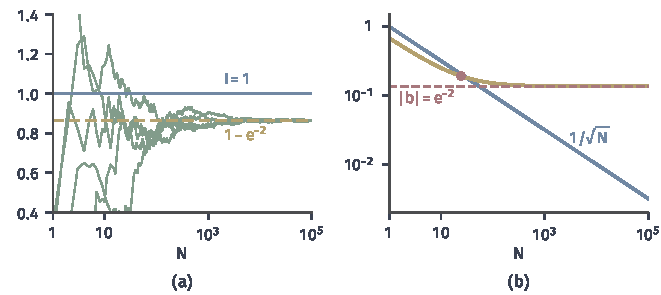
\includegraphics[width=112mm]{figures/07-probability/08-sampling-and-integration/matplotlib/mcerr-approx-bias/figure.pdf}
 \caption{截断程序$\min\{X,2\}$估计$\mathbb{E}[X]=1$，$X\sim\operatorname{Exp}(1)$，横轴为对数刻度。(a)五次运行的运行平均（绿线，种子$3116$至$3120$），蓝线为$I=1$，黄色虚线为$\tilde{\pi}$下的均值$1-\mathrm{e}^{-2}$；(b)均方根误差的精确值：蓝线为精确程序的$1/\sqrt{N}$，黄线为截断程序的$\sqrt{b^{2}+0.4403/N}$，红色虚线为$\lvert b\rvert=\mathrm{e}^{-2}$，红点标出方差项等于$b^{2}$的$N\approx24$。}
 \label{fig:mcerr-approx-bias}
\end{BookInlineFigure}

\paragraph{有界被积函数}
偏差无法从样本中读出，只能从$\tilde{\pi}$与$\pi$的差别估计出来。第~\ref{chap:distribution-comparison}章的总变差正好衡量这种差别：对有界的$f$，记$\operatorname{osc}(f)=\sup f-\inf f$，那里证明了
\begin{equation}
 \lvert b\rvert=\bigl\lvert\mathbb{E}_{\tilde{\pi}}[f]-\mathbb{E}_{\pi}[f]\bigr\rvert\leq\operatorname{osc}(f)\,d_{\mathrm{TV}}(\tilde{\pi},\pi)\leq2\sup\lvert f\rvert\,d_{\mathrm{TV}}(\tilde{\pi},\pi) .
 \label{eq:mcerr-tv-bound}
\end{equation}
所以只要知道近似分布与目标的总变差，就同时控制了所有有界被积函数的偏差。

截断程序的总变差可以直接算出。$\tilde{\pi}$在$[0,2)$上与$\pi$有相同的密度，把$\pi$在$(2,\infty)$上的质量$\mathrm{e}^{-2}$全部堆到点$2$上，如图~\ref{fig:mcerr-tv-bias}(a)。对任一事件$A$，差别只来自$A$与$\{2\}$、$(2,\infty)$的交，所以
\[
 \lvert\tilde{\pi}(A)-\pi(A)\rvert\leq\mathrm{e}^{-2},
\]
取$A=(2,\infty)$时等号成立，所以
\[
 d_{\mathrm{TV}}(\tilde{\pi},\pi)=\mathrm{e}^{-2} .
\]
对$f=\mathbf{1}_{\{x>2\}}$，$\operatorname{osc}(f)=1$，偏差恰为$-\mathrm{e}^{-2}$，式~\eqref{eq:mcerr-tv-bound}取到等号；对$f=\mathbf{1}_{\{x>1\}}$，截断不改变事件$\{X>1\}$，偏差为零。

\paragraph{无界被积函数}
对无界的$f$，总变差小并不能保证偏差小。设$\varepsilon\in(0,1)$，$c>1$，令近似分布为
\[
 \tilde{\pi}_{\varepsilon}=(1-\varepsilon)\,\pi+\varepsilon\,\delta_{c},\qquad \pi=\operatorname{Exp}(1) ,
\]
即以概率$1-\varepsilon$正常生成，以概率$\varepsilon$输出一个远处的值$c$。对任一事件$A$，
\[
 \lvert\tilde{\pi}_{\varepsilon}(A)-\pi(A)\rvert=\varepsilon\,\lvert\delta_{c}(A)-\pi(A)\rvert\leq\varepsilon ,
\]
所以$d_{\mathrm{TV}}\leq\varepsilon$。对$f(x)=x$，偏差却是$\varepsilon(c-1)$。取$c=1/\varepsilon^{2}$，总变差趋于零时偏差$1/\varepsilon-\varepsilon$趋于无穷。

图~\ref{fig:mcerr-tv-bias}(b)对照了这两种情形：有界的$f$的偏差随$\varepsilon$线性缩小，$f(x)=x$的偏差反而增大。问题出在少量质量被放到了很远的地方。总变差只问“同一事件的概率差多少”，不问质量移到了哪里；无界函数却对远处的质量非常敏感。

\begin{BookInlineFigure}
 \centering
 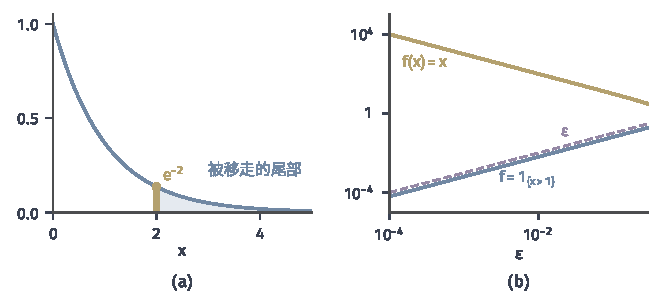
\includegraphics[width=112mm]{figures/07-probability/08-sampling-and-integration/matplotlib/mcerr-tv-bias/figure.pdf}
 \caption{总变差与积分偏差。(a)$\operatorname{Exp}(1)$的密度（蓝线）；截断程序把浅蓝区域中的尾部质量移到点$2$，形成质量为$\mathrm{e}^{-2}$的原子（黄色竖线，高度表示质量）。(b)近似分布$(1-\varepsilon)\operatorname{Exp}(1)+\varepsilon\delta_{1/\varepsilon^{2}}$的总变差不超过$\varepsilon$（紫色虚线）；蓝线为$f=\mathbf{1}_{\{x>1\}}$的偏差$\varepsilon(1-\mathrm{e}^{-1})$，黄线为$f(x)=x$的偏差$1/\varepsilon-\varepsilon$，双对数坐标。}
 \label{fig:mcerr-tv-bias}
\end{BookInlineFigure}

要让总变差重新起作用，需要控制两种分布在远处的质量。下面用二阶矩给出一个简单的结论。

\begin{lemma}[矩控制下的偏差界]
\label{lem:mcerr-moment-tv}
设$\mathbb{E}_{\pi}[f^{2}]\leq m$，$\mathbb{E}_{\tilde{\pi}}[f^{2}]\leq m$，记$d=d_{\mathrm{TV}}(\tilde{\pi},\pi)$。则
\begin{equation}
 \bigl\lvert\mathbb{E}_{\tilde{\pi}}[f]-\mathbb{E}_{\pi}[f]\bigr\rvert\leq4\sqrt{m\,d} .
 \label{eq:mcerr-moment-tv}
\end{equation}
\end{lemma}

\begin{proof}
$d=0$时两分布相同，结论成立。设$d>0$，固定截断水平$t>0$，把$f$分成有界部分与尾部：
\[
 f=f\,\mathbf{1}_{\{\lvert f\rvert\leq t\}}+f\,\mathbf{1}_{\{\lvert f\rvert>t\}} .
\]
有界部分的振幅不超过$2t$，由式~\eqref{eq:mcerr-tv-bound}，它在两分布下的期望差不超过$2td$。

尾部在$\lvert f\rvert>t$时满足$\lvert f\rvert\leq f^{2}/t$，所以对$\pi$与$\tilde{\pi}$都有
\[
 \bigl\lvert\mathbb{E}\bigl[f\,\mathbf{1}_{\{\lvert f\rvert>t\}}\bigr]\bigr\rvert\leq\frac{\mathbb{E}[f^{2}]}{t}\leq\frac{m}{t} .
\]
两分布下的尾部期望之差不超过$2m/t$。合起来，偏差不超过$2td+2m/t$。取$t=\sqrt{m/d}$，两项都等于$2\sqrt{md}$。
\end{proof}

证明里的截断水平体现了两种误差的折中：$t$越大，有界部分越宽，总变差的作用被放大；$t$越小，留在尾部的质量越多。界$4\sqrt{md}$随$d$按平方根缩小，比有界情形的线性缩小慢，这是为控制尾部付出的代价。对截断程序，$f(x)=x$在两分布下的二阶矩分别是$2$和$1.188$，取$m=2$，界为
\[
 4\sqrt{2\times0.1353}=2.081 ,
\]
远大于实际的$0.1353$，但它不依赖任何具体计算。对$\tilde{\pi}_{\varepsilon}$，二阶矩至少为$\varepsilon c^{2}=\varepsilon^{-3}$，代入后界的量级是$4/\varepsilon$，与实际偏差的量级一致：矩条件正好抓住了远处质量的作用。

\paragraph{近似转移}
用Markov链采样时，近似发生在转移这一步：理论上的转移核$K$以$\pi$为不变分布，实际程序执行的却是另一个核$\tilde{K}$。这时要先回答一个更基本的问题：$\tilde{K}$有没有不变分布，有的话它离$\pi$多远。链跑得再久，平均也只能趋向$\tilde{K}$自己的长期规律。

看一个可以算到底的例子。目标是$\pi=\mathcal{N}(0,1)$，某个由连续时间动态离散化得到的更新为
\[
 X^{(t+1)}=(1-h)X^{(t)}+\sqrt{2h}\,\xi^{(t+1)} ,
\]
其中$\xi^{(1)},\xi^{(2)},\dots$独立且服从$\mathcal{N}(0,1)$，与$X^{(0)}$独立，$h>0$是步长。若$X^{(t)}\sim\mathcal{N}(0,v)$，则$X^{(t+1)}\sim\mathcal{N}(0,(1-h)^{2}v+2h)$。令两者相等，
\[
 v=(1-h)^{2}v+2h,\qquad v=\frac{2h}{1-(1-h)^{2}}=\frac{2}{2-h},\qquad 0<h<2 .
\]
所以$0<h<2$时，$\mathcal{N}(0,2/(2-h))$是这个近似转移的不变分布，而$\pi$不是。

从任意$x$出发，展开递推得到
\[
 X^{(t)}=(1-h)^{t}x+\sum_{j=1}^{t}(1-h)^{t-j}\sqrt{2h}\,\xi^{(j)} ,
\]
它服从均值为$(1-h)^{t}x$、方差为$2h\sum_{j<t}(1-h)^{2j}$的高斯分布。$\lvert1-h\rvert<1$时，均值趋于零，方差趋于$v$，链确实趋向这个不变分布。取$h=0.5$，$v=4/3$。对$f(x)=x^{2}$，偏差为$4/3-1=1/3$；对有界的$f=\mathbf{1}_{\{\lvert x\rvert\leq1\}}$，
\[
 \mathbb{P}_{\mathcal{N}(0,4/3)}\bigl(\lvert X\rvert\leq1\bigr)=2\Phi\bigl(\sqrt{3}/2\bigr)-1=0.6135 ,
\]
而目标值是$2\Phi(1)-1=0.6827$，偏差为$-0.0692$。图~\ref{fig:mcerr-approx-chain}(b)中，$10^{5}$步的直方图贴合的是$\mathcal{N}(0,4/3)$，不是$\pi$。

$h\geq2$时，不变分布根本不存在。设$\mu$是不变分布，$\phi$是它的特征函数，则$X\sim\mu$与独立的$\xi$满足$(1-h)X+\sqrt{2h}\,\xi\sim\mu$，即
\[
 \phi(s)=\phi\bigl((1-h)s\bigr)\,\mathrm{e}^{-hs^{2}} .
\]
记$c=\lvert1-h\rvert\geq1$。特征函数的模不超过$1$，把上式反复代入$k$次，
\[
 \lvert\phi(s)\rvert\leq\exp\Bigl(-hs^{2}\sum_{j=0}^{k-1}c^{2j}\Bigr)\leq\mathrm{e}^{-khs^{2}} .
\]
令$k\to\infty$，对每个$s\neq0$得$\phi(s)=0$。这与特征函数在$0$处连续且$\phi(0)=1$矛盾。图~\ref{fig:mcerr-approx-chain}(a)画出不变方差$2/(2-h)$，它在$h\to2$时趋于无穷。

\begin{BookInlineFigure}
 \centering
 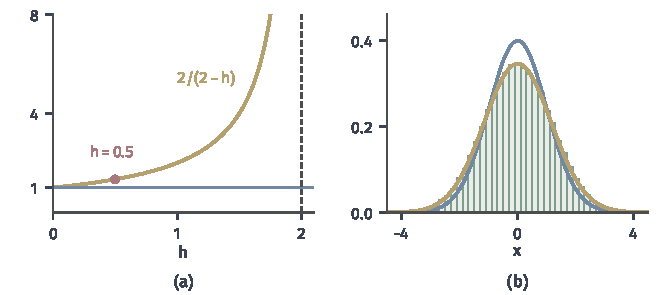
\includegraphics[width=112mm]{figures/07-probability/08-sampling-and-integration/matplotlib/mcerr-approx-chain/figure.pdf}
 \caption{近似转移$X'=(1-h)X+\sqrt{2h}\,\xi$，目标为$\mathcal{N}(0,1)$。(a)不变分布的方差$2/(2-h)$（黄线）与目标方差$1$（蓝线），灰色虚线为$h=2$，红点为$h=0.5$；(b)$h=0.5$时从$0$出发运行$10^{5}$步的直方图（绿色，种子$3121$），蓝线为目标密度，黄线为不变分布$\mathcal{N}(0,4/3)$的密度。}
 \label{fig:mcerr-approx-chain}
\end{BookInlineFigure}

这个例子显示了近似链需要分两步检查。先确认近似转移存在不变分布、并且链会趋向它；再估计它与$\pi$的差，必要时减小步长或用第~\ref{chap:sample-generation}章的Metropolis接受步骤校正，使$\pi$恢复为精确的不变分布。两步都与运行长度无关。
